% Hlavicka pro protokoly z fyzikalniho praktika.
% Verze pro: LaTeX
% Verze hlavicky: 22. 2. 2007
% Autor: Ustav fyziky kondenzovanych latek
% Ke stazeni: www.physics.muni.cz/ufkl/Vyuka/
% Licence: volne k pouziti, nejlepe k vcasnemu odevzdani protokolu z Vaseho mereni.


\documentclass[czech,11pt,a4paper]{article}
\usepackage[T1]{fontenc}
\usepackage{graphicx, animate}
\usepackage{mathtools}
\usepackage{amssymb}
\usepackage{amsthm}
\usepackage{thmtools}
\usepackage{xcolor}
\usepackage{nameref}
\usepackage{babel}
\usepackage{hyperref}
\usepackage{multicol}
\usepackage[export]{adjustbox}
\usepackage{subcaption}
\usepackage{caption}
\usepackage{multirow}
\usepackage{float}
\usepackage{placeins}
\usepackage{biblatex}
\graphicspath{ {./images/} }




%%% Nemente:
\usepackage[margin=2cm]{geometry}
\newtoks\jmenopraktika \newtoks\jmeno \newtoks\datum
\newtoks\obor \newtoks\skupina \newtoks\rocnik \newtoks\semestr
\newtoks\cisloulohy \newtoks\jmenoulohy
\newtoks\tlak \newtoks\teplota \newtoks\vlhkost
%%% Nemente - konec.


%%%%%%%%%%% Doplnte pozadovane polozky:

\jmenopraktika={Fyzikální praktikum 2}  % nahradte jmenem vaseho predmetu
\jmeno={Teodor Duraković}            % nahradte jmenem mericiho
\datum={16.~prosince 2024}        % nahradte datem mereni ulohy
\obor={F}                     % nahradte zkratkou vami studovaneho oboru
\skupina={Po 14:00}            % nahradte dobou vyuky vasi seminarni skupiny
\rocnik={II}                  % nahradte rocnikem, ve kterem studujete
\semestr={III}                 % nahradte semestrem, ve kterem studujete

\cisloulohy={11}               % nahradte cislem merene ulohy
\jmenoulohy={Interference a difrakce světla} % nahradte jmenem merene ulohy

\tlak={1000}                   % nahradte tlakem pri mereni (v hPa)
\teplota={21.3}               % nahradte teplotou pri mereni (ve stupnich Celsia)
\vlhkost={27}               % nahradte vlhkosti vzduchu pri mereni (v %)

%%%%%%%%%%% Konec pozadovanych polozek.


%%%%%%%%%%% Uzitecne balicky:

%%%%%% Zamezeni parchantu:
\widowpenalty 10000 \clubpenalty 10000 \displaywidowpenalty 10000
%%%%%% Parametry pro moznost vsazeni vetsiho poctu obrazku na stranku
\setcounter{topnumber}{3}	  % max. pocet floatu nahore (specifikace t)
\setcounter{bottomnumber}{3}	  % max. pocet floatu dole (specifikace b)
\setcounter{totalnumber}{6}	  % max. pocet floatu na strance celkem
\renewcommand\topfraction{0.9}	  % max podil stranky pro floaty nahore
\renewcommand\bottomfraction{0.9} % max podil stranky pro floaty dole
\renewcommand\textfraction{0.1}	  % min podil stranky, ktery musi obsahovat text
\intextsep=8mm \textfloatsep=8mm  %\intextsep pro ulozeni [h] floatu a \textfloatsep pro [b] or [t]

% Tecky za cisly sekci:
\renewcommand{\thesection}{\arabic{section}.}
\renewcommand{\thesubsection}{\thesection\arabic{subsection}.}
\renewcommand{\thesubsubsection}{\thesubsection\arabic{subsubsection}.}
% Jednopismenna mezera mezi cislem a nazvem kapitoly:
\makeatletter \def\@seccntformat#1{\csname the#1\endcsname\hspace{1ex}} \makeatother


%%%%%%%%%%%%%%%%%%%%%%%%%%%%%%%%%%%%%%%%%%%%%%%%%%%%%%%%%%%%%%%%%%%%%%%%%%%%%%%
%%%%%%%%%%%%%%%%%%%%%%%%%%%%%%%%%%%%%%%%%%%%%%%%%%%%%%%%%%%%%%%%%%%%%%%%%%%%%%%
% Zacatek dokumentu
%%%%%%%%%%%%%%%%%%%%%%%%%%%%%%%%%%%%%%%%%%%%%%%%%%%%%%%%%%%%%%%%%%%%%%%%%%%%%%%
%%%%%%%%%%%%%%%%%%%%%%%%%%%%%%%%%%%%%%%%%%%%%%%%%%%%%%%%%%%%%%%%%%%%%%%%%%%%%%%

\begin{document}
	
	%%%%%%%%%%%%%%%%%%%%%%%%%%%%%%%%%%%%%%%%%%%%%%%%%%%%%%%%%%%%%%%%%%%%%%%%%%%%%%%
	% Nemente:
	%%%%%%%%%%%%%%%%%%%%%%%%%%%%%%%%%%%%%%%%%%%%%%%%%%%%%%%%%%%%%%%%%%%%%%%%%%%%%%%
	\thispagestyle{empty}
	
	{
		\begin{center}
			\sf 
			{\Large Ústav fyzikální elektroniky Přírodovědecké fakulty Masarykovy univerzity} \\
			\bigskip
			{\huge \bfseries FYZIKÁLNÍ PRAKTIKUM} \\
			\bigskip
			{\Large \the\jmenopraktika}
		\end{center}
		
		\bigskip
		
		\sf
		\noindent
		\setlength{\arrayrulewidth}{1pt}
		\begin{tabular*}{\textwidth}{@{\extracolsep{\fill}} l l}
			\large {\bfseries Zpracoval:}  \the\jmeno & \large  {\bfseries Naměřeno:} \the\datum\\[2mm]
			\large  {\bfseries Obor:} \the\obor  \hspace{40mm}  {\bfseries Skupina:} \the\skupina %
			%{\bfseries Ročník:} \the\rocnik \hspace{5mm} {\bfseries Semestr:} \the\semestr  
			&\large {\bfseries Testováno:}\\
			\\
			\hline
		\end{tabular*}
	}
	
	\bigskip
	
	{
		\sf
		\noindent \begin{tabular}{p{3cm} p{0.6\textwidth}}
			\Large  Úloha č. {\bfseries \the\cisloulohy:} \par
			\smallskip
			$T=\the\teplota$~$^\circ$C \par
			$p=\the\tlak$~hPa \par
			$\varphi=\the\vlhkost$~\%
			&\Large \bfseries \the\jmenoulohy  \\[2mm]
		\end{tabular}
	}
	
	\vskip1cm
	
	%%%%%%%%%%%%%%%%%%%%%%%%%%%%%%%%%%%%%%%%%%%%%%%%%%%%%%%%%%%%%%%%%%%%%%%%%%%%%%%
	% konec Nemente.
	%%%%%%%%%%%%%%%%%%%%%%%%%%%%%%%%%%%%%%%%%%%%%%%%%%%%%%%%%%%%%%%%%%%%%%%%%%%%%%%
	
	%%%%%%%%%%%%%%%%%%%%%%%%%%%%%%%%%%%%%%%%%%%%%%%%%%%%%%%%%%%%%%%%%%%%%%%%%%%%%%%
	%%%%%%%%%%%%%%%%%%%%%%%%%%%%%%%%%%%%%%%%%%%%%%%%%%%%%%%%%%%%%%%%%%%%%%%%%%%%%%%
	% Zacatek textu vlastniho protokolu
	%%%%%%%%%%%%%%%%%%%%%%%%%%%%%%%%%%%%%%%%%%%%%%%%%%%%%%%%%%%%%%%%%%%%%%%%%%%%%%%
	%%%%%%%%%%%%%%%%%%%%%%%%%%%%%%%%%%%%%%%%%%%%%%%%%%%%%%%%%%%%%%%%%%%%%%%%%%%%%%%
	
	\begin{multicols}{2}
		
	
	\section{Teorie}
	\section*{Index lomu}
	Ve vakuu se světlo pohybuje rychlostí
	
	\begin{equation}
		c_{0}=2,99792458 \cdot 10^{8} \mathrm{~m} / \mathrm{s}
	\end{equation}
	
	
	Pokud se světlo šíří dielektrickým prostředím (plyn, tekutina, sklo nebo jiná průhledná pevná látka), jeho rychlost se sníží na
	
	
	\begin{equation}
		c=\frac{c_{0}}{n},
	\end{equation}
	
	
	kde $n$ je index lomu. Index lomu je důležitou charakteristikou prostředí, která navíc závisí na barvě, tj. vlnové délce $\lambda$ světla, stejně jako na teplotě a tlaku. Poslední jmenovaná závislost je nejvíce výrazná pro plyny. Typické hodnoty jsou $n=1,33$ pro vodu, $n=1,4$ až 2,0 pro různé typy skel, zatímco pro plyny (včetně vzduchu) je odchylka indexu lomu od jedničky $n-1$ řádově $10^{-4}$.
	
	\section*{Rovinné monochromatické vlny}
	Světlo je (v rámci vlnového pojetí světla) elektromagnetická vlna, která je charakterizována elektrickým polem $\boldsymbol{E}(\boldsymbol{r}, t)$, nazývaným optické pole, které závisí na čase $t$ a polohovém vektoru v prostoru $\boldsymbol{r}$. Světlo vyzařované laserem lze v dobrém přiblížení popsat jako rovinnou monochromatickou vlnu. Uvažujeme-li takovou vlnu, která se šíří podél osy $x$, časová a prostorová závislost optického pole je dána vztahem
	
	\begin{equation}
		E(x, t)=E_{0} \cos \left(k x-\omega t+\phi_{0}\right),
	\end{equation}
	
	
	kde $\omega$ je úhlová frekvence, $k$ je úhlové vlnové číslo a $\phi_{0}$ je počáteční fáze (fázová konstanta). Úhlová frekvence a úhlové vlnové číslo jsou svázány vztahem
	
	\begin{equation}
		k=\frac{\omega}{c}=n \frac{\omega}{c_{0}}=n k_{0}
	\end{equation}
	
	
	kde
	
	\begin{equation}
		k_{0}=\frac{\omega}{c_{0}}=\frac{2 \pi \nu}{c_{0}}=\frac{2 \pi}{\lambda_{0}}
	\end{equation}
	
	
	je (úhlové) vlnové číslo ve vakuu a
	
	\begin{equation}
		\lambda_{0}=\frac{c_{0}}{\nu}
	\end{equation}
	
	
	je vlnová délka ve vakuu a $\nu$ je frekvence. Z tohoto výrazu je patrné, že se vlnová délka světla změní na
	
	\begin{equation}
		\lambda=\frac{\lambda_{0}}{n}
	\end{equation}
	
	
	pokud se šíří prostředím s indexem lomu $n \neq 1$, zatímco frekvence $\nu$ světla se nezmění.
	
	\section*{Reprezentace a šíření vlny}
	Uvažme rovinnou vlnu v čase $t=0$ šířící se ve směru osy $x$
	
	\begin{equation}
		E(x)=E_{0} \cos (k x),
	\end{equation}
	
	
	kde $\Phi=k x$ se nazývá prostorová fáze vlny. Tato vlna může být graficky reprezentována funkcí $E(x)$ (viz obr. 1 $)$ ) nebo vlnoplochami, což jsou roviny kolmé na vlnový vektor $\boldsymbol{k}$ (obr. 1b)), jehož velikost je rovna úhlovému vlnovému číslu.\\
	
	\begin{figure}[H]
			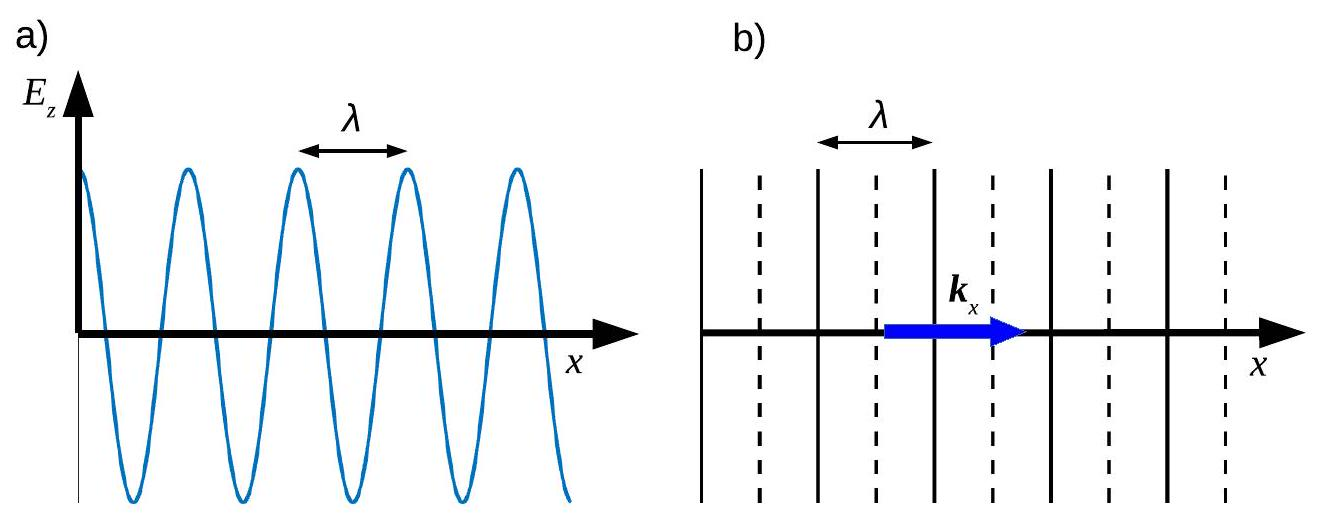
\includegraphics[width=0.95\linewidth, center]{2024_12_20_2ef48a0ed8e6cd108eb0g-02}
			\caption{Grafické reprezentace elektromagnetické rovinné monochromatické vlny šířící se podél osy $x$ pomocí a) funkce intenzity elektrického pole $E(x)$ a b) pomocí vlnoploch, které jsou rovinami kolmými k vlnovému vektoru $\boldsymbol{k}$ a vzájemně vzdálené o vlnovou délku $\lambda$.}
	\end{figure}

	
	
	Vlnoplochy prochází body prostoru, ve kterých optické pole $E(x)$ nabývá určité hodnoty. V našem případě jsme je reprezentovali spojitými čarami v bodech, kde $E(x)$ dosahuje svého maxima $E_{0}$ a přerušovanými čarami v bodech, kde funkce dosahuje minima $-E_{0}$. Sousední vlnoplochy odpovídající stejné hodnotě $E(x)$ (tj. zde maximům či minimům) jsou vzájemně vzdáleny o vlnovou délku $\lambda$. Šíření vlny prostorem by odpovídal pohyb obou reprezentací vlny na obr. 1 rychlostí $c$ podél osy $x$. V bodě $x+\Delta x$, je prostorová fáze vlny ( tj . argument funkce cos v (8)
	
	\begin{equation}
		\Phi=k(x+\Delta x)=k x+k \Delta x=k x+\Delta \Phi
	\end{equation}
	
	
	a mluvíme o přírůstku fáze vlny vůči bodu $x$ o
	
	\begin{equation}
		\Delta \Phi=k \Delta x=n k_{0} \Delta x
	\end{equation}
	
	
	na dráze $\Delta x$. Zatímco $\Delta x$ nazýváme geometrickou dráhou, $n \Delta x$ se nazývá dráhou optickou.
	
	\section*{Intenzita rovinné vlny}
	Intenzita (též plošná hustota zářivého toku) $I$ rovinné vlny (3) je přímo úměrná časově průměrovanému kvadrátu intenzity elektrického pole [6]
	
	\begin{equation}
		I=\varepsilon_{0} c\left\langle E(x, t)^{2}\right\rangle_{t}=\frac{\varepsilon_{0} c}{2} E_{0}^{2}
	\end{equation}
	
	
	Jednotkou intenzity jsou $\mathrm{W} / \mathrm{m}^{2}$. Intenzita rovinné vlny je úměrná kvadrátu amplitudy $E_{0}$ vlnového pole, ale je nezávislá na veličinách $k, \omega, x$ a $t$.
	
	\section*{Michelsonův interferometr}
	V této úloze bude využito Michelsonova interferometru (viz schéma na obr. 2). Svazek světla z laseru $(\mathrm{ZS})^{1}$ dopadá na dělič svazku (DS) a elektromagnetická vlna je rozdělena do dvou větví interferometru vedoucím k zrcátku Z1 (příp. vzorku V), resp. k zrcátku 2 (Z2). Dělič svazku je polopropustné zrcátko připravené a instalované ideálně tak, že je intenzita prošlého svazku rovna intenzitě svazku odraženého. Každá ze dvou vzniklých vln se šíří k jednomu ze zrcátek, které vlnu odráží ve směru proti vlně dopadající případně s malou úhlovou odchylkou. Kvůli lepší vizualizaci jsou na obr. 2 vlny dopadající a na zrcátku odražená stranově mínně posunuty. Po odrazu na zrcátkách Z1/V, resp. Z2 vlny postupují zpĕt směrem na dĕlič svazku, který opět propustí polovinu intenzity svazku a druhou polovinu odrazí. Pro zjednodušení jsou však na obrázku zobrazeny pouze pro nás relevantní části svazku postupující dále k projekčnímu stínítku (PS).\\
	
	\begin{figure}[H]
			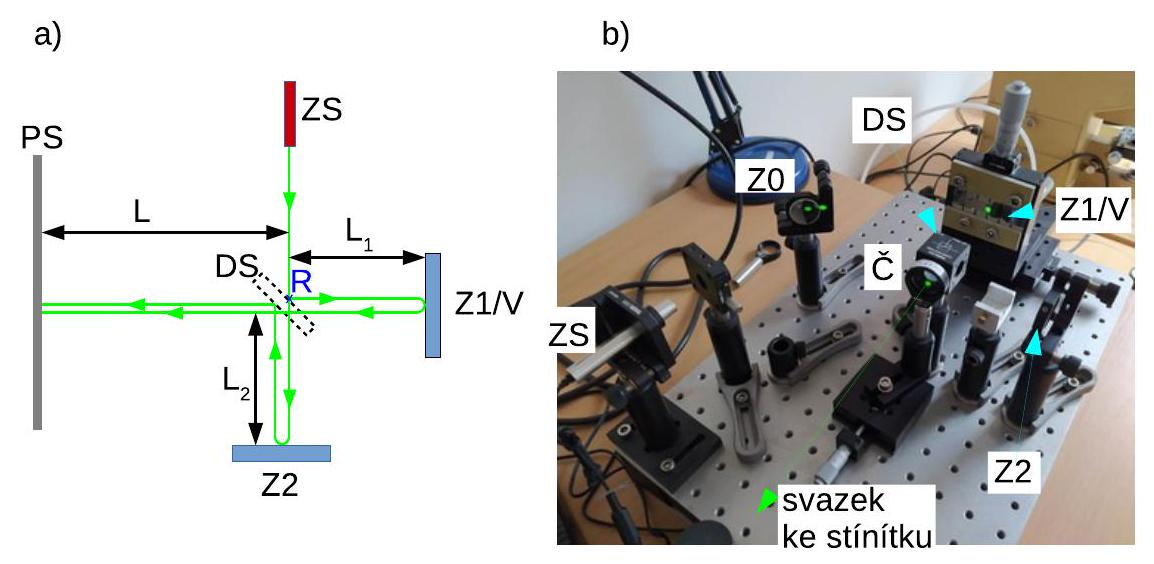
\includegraphics[max width=0.95\linewidth, center]{2024_12_20_2ef48a0ed8e6cd108eb0g-03}
			\caption{a) Schéma Michelsonova interferometru s vyznačenými trajektoriemi vln. b) Realizace Michelsonova interferometru v praktiku. Části interferometru: zdroj světla (laser, ZS), pomocné zrcátko (Z0), dělič svazku (polopropustné zrcátko, DS), zrcátko č. 1 nebo vzorek (Z1/V), zrcátko č. 2 (Z2), spojná čočka zvĕtšující svazek (Č) a projekční stínítko (PS). Dále jsou ve schématu a) vyznačeny geometrické dráhy v první a druhé větvi interferometru $\left(L_{1}\right.$, resp. $\left.L_{2}\right)$ a ve společné větvi mezi dĕličem svazku a stínítkem (L).}
	\end{figure}

	
	Fáze, kterou nabyde vlna procházející první vĕtví interferometru na trajektorii od referenčního bodu R až ke stínítku PS (tj. trajektorii DS (reflexe v R) $\rightarrow \mathrm{Z1} \rightarrow \mathrm{DS}$ (průchod) $\rightarrow$ PS) je
	
	\begin{equation}
		\Phi_{1}=k\left(2 L_{1}+L\right)+\Phi_{\mathrm{LS}},
	\end{equation}
	
	
	\footnotetext{${ }^{1} \mathrm{~V}$ praktiku použitý laserový svazek můžeme ve velice dobrém přibližení chápat jako prostorově omezenou rovinnou vlnu.
	}
	kde $\Phi_{\text {LS }}$ je fáze nabytá při odrazu na DS a průchodu DS. Podobně část vlny, která prochází druhou větví interferometru od R k PS (tj. po trajektorii DS (průchod v R) $\rightarrow \mathrm{Z} 2 \rightarrow \mathrm{DS}$ (odraz) $\rightarrow \mathrm{PS}$ ), nabyde fázi
	
	\begin{equation}
		\Phi_{2}=k\left(2 L_{2}+L\right)+\Phi_{\mathrm{LS}}
	\end{equation}
	
	
	Protože každá z vln se jednou odráží a jednou prochází DS , je člen $\Phi_{\mathrm{LS}}$ pro obě vlny (tedy v obou vztazích (12) a (13) identický. Pokud je amplituda vlny dopadající na DS z ZS v referenčním bodě R $E_{0}$, jsou optická pole diskutovaných dvou vln na stínítku PS dané
	
	\begin{equation}
		E_{1}=\frac{E_{0}}{2} \cos \left(\Phi_{1}-\omega t\right), \text { resp. } E_{2}=\frac{E_{0}}{2} \cos \left(\Phi_{2}-\omega t\right)
	\end{equation}
	
	kde jsme započetli fakt, že každý odraz na DS, příp. průchod přes DS, zmenší amplitudu svazku o faktor $\sqrt{2}$. Celková intenzita výsledného vlnového pole na PS je
	
	
	\begin{equation}
		\left.I_{\mathrm{tot}}=\varepsilon_{0} c\langle | E_{1}+\left.E_{2}\right|^{2}\right\rangle_{t}
	\end{equation}
	
	
	kde $\left\rangle_{t}\right.$ opět značí průměrování přes čas. Po krátkém výpočtu dostáváme výsledný vztah pro intenzitu
	
	\begin{align}
		I_{\mathrm{tot}} &=\frac{I_{0}}{2}\left[1+\cos \left(\Phi_{1}-\Phi_{2}\right)\right]= 
	\end{align}
	\begin{align*}
		& =\frac{I_{0}}{2}\left[1+\cos \left(2 k\left(L_{1}-L_{2}\right)\right)\right]= \\
		& =\frac{I_{0}}{2}\left[1+\cos \left(4 \pi \frac{n_{\mathrm{vz}} L_{1}-n_{\mathrm{vz}} L_{2}}{\lambda_{0}}\right)\right]
	\end{align*}
	
	
	kde $n_{\mathrm{vz}}$ je index lomu vzduchu. Tyto rovnice ukazují, že interferenční obraz na PS závisí pouze na rozdílu fází $\Delta \Phi=\Phi_{1}-\Phi_{2}$ vln přícházejících ze dvou větví interferometru nebo, ekvivalentně, na rozdílu příslušných dvou optických drah. Vidíme, že pokud budeme mĕnit rozdíl optických drah, můžeme měnit intenzitu světla zaznamenávanou na PS mezi $I_{\mathrm{tot}}=0$ a $I_{\mathrm{tot}}=I_{0}$. Na tomto principu budou založena měření využívající interferenci v tomto praktiku.
	
	\section*{Princip měření fáze}
	Pokud se dvě interferující vlny šíří přesně ve stejném směru, uvidíme na stínítku jedinou skvrnu homogenní intenzity. Intenzita se bude měnit periodicky podle rovnice 16, pokud budeme měnit relativní fázi, tedy rozdíl geometrických drah, těchto dvou vln. Pokud změníme rozdíl fází $\Delta \Phi=\Phi_{1}-\Phi_{2}$ právě o $2 \pi$, budeme pozorovat opět stejnou intenzitu skvrny (např. přejdeme od maxima k maximu intenzity). Nicméně, pokud se budou dvě vlny dopadající na stínítko šířit vzájemně v poněkud odlišném směru, budeme pozorovat střídavě několik světlých a tmavých proužků, nazývaných interferenční proužky. Na obr. 3 jsou vyobrazena schémata optických polí dvou různobĕžných rovinných vln a výsledných interferenčních obrazců pro dva různé úhly mezi interferujícími rovinnými vlnami. Optická pole jsou vyobrazena v určitý okamžik, kdy je maximum optického pole č. 2 právě totožné s povrchem stínítka. Maxima intenzity vznikají v bodech stínítka, kde jsou fáze obou vln na stínítku stejné, tedy v zobrazeném případě tam, kde optická pole vykazují maxima. Ta jsou v momentce ve schématech vyznačena opět plnou čarou. Ve skutečnosti se vlny pohybují rychlostí světla, ale body na stínítku, kde mají vlny stejnou fázi, se nepohybují a tím pádem zůstává interferenční obraz statický. Pokud na druhou stranu změníme fázi jedné z vln (např. posuneme zrcátko Z1 na obr. 2 směrem ke stínítku), interferenční obraz se posune. Situace na obr. 3 odpovídá případu, kdy jsou zrcátko Z2 a stínítko PS na obr. 2 orientovány normálami podél dopadajícího svazku procházejícího větví č. 2 Michelsonova interferometru, zatímco normála k Z1 je otočena kolem horizontální osy.
	
	Z analýzy schématu interferujících vlnových polí v blízkosti stínítka na obr. 4 získáme vztah mezi úhlem, který svírají interferující vlny a vzdáleností sousedních interferenčních proužků.\\
	
	\begin{figure}[H]
			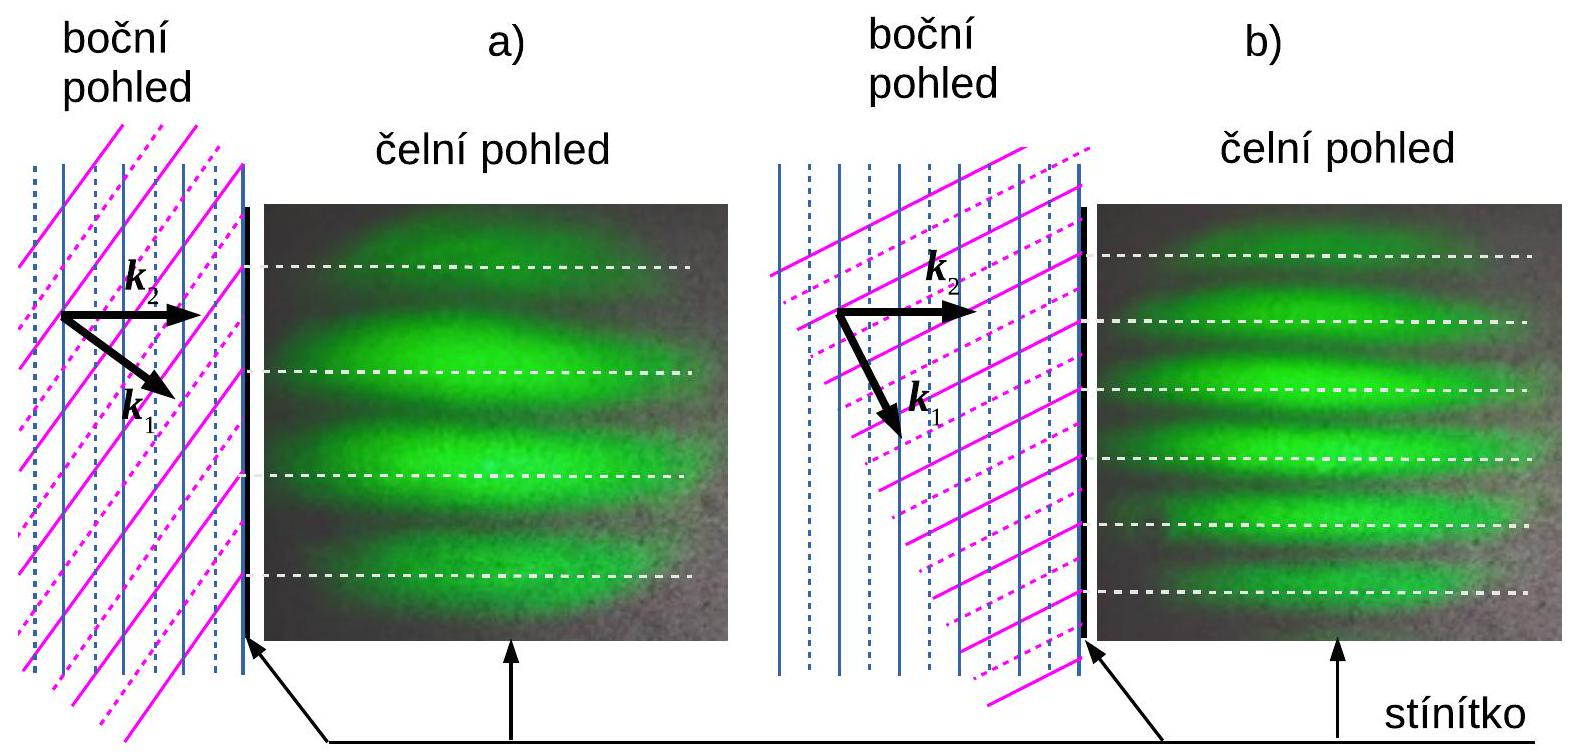
\includegraphics[max width=0.95\linewidth, center]{2024_12_20_2ef48a0ed8e6cd108eb0g-05}
			\caption{Boční pohledy na interferující optická pole dvou různoběžných rovinných vln šírirících se v různých směrech a čelní pohledy na výsledné interferenční proužky na stínítku (fotografie). Schémata optických polí a interferenční obrazce jsou vyobrazeny pro a) menší a b) větší úhel mezi směry šíření rovinných vln. Směry šíření jsou dány směry vlnových vektorů $\boldsymbol{k}_{1}$ a $\boldsymbol{k}_{2}$. Intenzivní interferenční proužky vznikají v bodech, kde mají vlny na stínítku stejnou fázi, což jsou ve vyobrazeném případě průsečíky maxim optických polí vyznačených plnými čarami.}
	\end{figure}

	
	
	Konkrétně se zaměřme na pravoúhlý trojúhelník, jehož vrcholy A a B leží v bodech sousedních interferenčních maxim a vrchol C je kolmou projekcí bodu A na sousední vlnoplochu, odpovídající následujícímu maximu vlny 2 . Odvěsna AC tohoto trojúhlelníku má délku rovnou vlnové délce světla $\lambda$, délka přepony AB je vzdálenost maxim $x_{1}$, a úhel protilehlý k odvěsně AC je roven úhlu mezi směry šíření vln 1 a 2 , označenému $2 \theta \|^{2}$ Odtud dostáváme pro vzdálenost mezi difrakčními maximy
	
	
	\begin{equation}
		x_{1}=\frac{\lambda}{\sin (2 \theta)}
	\end{equation}
	
	
	Na tomto místě poznamenejme, že úhly mezi směry šíření vln 1 a 2 na obr. 3 a 4 byly oproti experimentu v praktiku značně zveličeny. Úhly jsou v obrázku přizpůsobeny tomu, aby bylo možné zároveň viditelně zobrazit vzdálenosti vlnoploch $\lambda$ (řádově stovky nm pro viditelné světlo) a vzdálenosti interferenčních maxim $x$, které jsou řádu jednotek mm. Dosadíme-li do vztahu (17) např. vzdálenost proužků 4 mm a vlnovou délku zeleného svĕtla $\lambda=530 \mathrm{~nm}$, dostáváme pro úhel mezi směry șíření vln $2 \theta \approx 8 \cdot 10^{-30} \approx 0,5^{\prime}$. Úhly $2 \theta$ mezi směry šíření rovinných vln vycházejících z větví 1 a 2 Michelsonova interferometru v praktiku budou tedy řádově desetiny až jednotky úhlové minuty.
	
	\section*{Měření tloušťky tenké vrstvy pomocí interference}
	\section*{Princip měření}
	Měření bude provedeno pomocí Michelsonova interferometru (viz obr. 5 a 2 a). Jako vzorek použijeme tenkou vrstvu hliníku (TV, viz obr. 5b)) nanesenou na skleněném podložním skličcku ( S ). Vrstva byla při depozici rozdělena pomocí masky na řadu obdélníků oddělených mezerami. Navíc je přes tuto tenkou vrstvu a mezery podél délky vzorku nanesena krycí vrstva (KV) z hliníku (příp. z Au), u které předpokládáme stejnou tloušťku v oblastech TV i na skle (obr.
	
	\footnotetext{${ }^{2} \mathrm{~V}$ teorii rozptylu se konvenčně označuje úhel mezi dvěma interferujícími nebo difraktujícími vlnami $2 \theta$.
	}
	\begin{figure}[H]
			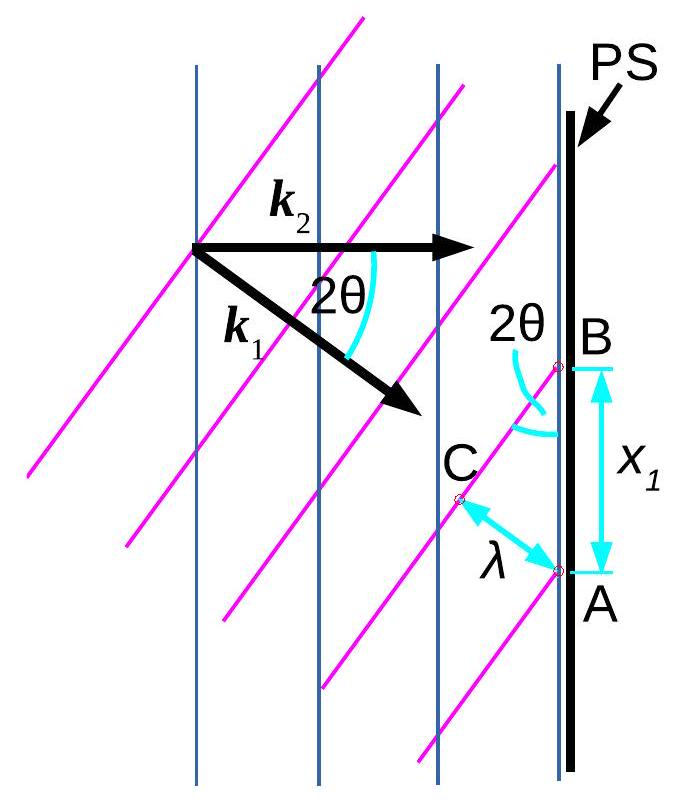
\includegraphics[max width=0.95\linewidth, center]{2024_12_20_2ef48a0ed8e6cd108eb0g-06}
			\caption{Schématické zobrazení interferujících vlnových polí z obr. 3a) v blízkosti stínítka (PS) v boční projekci. Pro přehlednost jsou zobrazeny pouze vlnoplochy odpovídající maximům optických polí vln 1 a 2 (fialové, resp. modré plné čáry). Na obrázku byla opět znázorněna situace v momentě, kdy je maximum pole 2 právě totožné s povrchem stínítka. Úhel mezi směry šíření vlnových polí je $2 \theta$, vzdálenost interferenčních proužků na stínítku je $x_{1}$.}
	\end{figure}

	
	5 f)). Účelem použití KV je dosáhnout vysoké odrazivosti vzorku nad TV i mezerami, což je potřebné k obdržení intenzivního a kontrastního interferenčního obrazce. Zatímco sklo má pro viditelné světlo při kolmém dopadu odrazivost řádově jednotek procent, odrazivost kovů je ve vyšších desítkách procent (pro Al více jak $90 \%$ ).
	
	V experimentu bude vzorek umístěn v první větvi interferometru (obr. 2b)) tak, aby svazek dopadal na KV částečně nad TV (KV-TV) a částečně v oblasti mezery na KV na skle (KV-S), kde je krycí vrstva přímo na skle, (viz obr. 6a)). Vlna odražená v oblasti KV-S musí urazit geometrickou dráhou o dvojnásobek tlouštky vrstvy $t$ větší oproti vlně odražené na KV-TV ( $L_{1, \mathrm{~S}^{-}}$ $\left.L_{1, \mathrm{TV}}=2 t\right)$ (viz obr. 6c)). Obě vlny interferují s optickým polem vlny odražené na referenčním zrcátku Z2. Přitom vlny odražené na vzorku svírají s vlnou od Z2 nenulový (v experimentu malý, $2 \theta<10^{\prime}$ ) úhel ve vertikální rovině. Díky odlišné geometrické dráze $s=2 t$ části vlny po odrazu na KV-TV a KV-S ke stínítku budou interferenční obrazce od těchto dvou vln vertikálně posunuty (obr. 6b)).
	
	Vztah mezi tloušťkou vrstvy $t$ a vertikálním posunem interferenčních obrazců $x_{2}$ dostaneme z analýzy schématu optických polí v blízkosti stínítka na obr. 7. Jak plyne ze schématu, pro jednoznačné určení tloušťky vrstvy $t$ musí být rozdíl optických drah vln ze vzorku menší než vlnová délka světla, tedy $t=s / 2<\lambda / 2$. Z podobnosti trojúhelníků ABC a AED dostáváme pro tloušťku vrstvy
	
	
	\begin{equation}
		t=\frac{x_{2}}{x_{1}} \frac{\lambda}{2}
	\end{equation}
	
	
	kde $x_{1}$ je opět vzdálenost nejbližších interferenčních maxim od vlny odražené na KV-TV. Vzhledem k tomu, že relativní nejistota měření vzdálenosti interferenčních proužků v experimentu bude o řád či více větší než odchylka indexu lomu vzduchu od jedničky, můžeme v 18 aproximovat vlnovou délku světla laseru ve vzduchu vakuovou vlnovou délkou $\lambda \approx \lambda_{0}$.\\
	
	\section*{Postup měření}
	Zapněte laser (zelený laser vlnové délky $\lambda=531,2 \mathrm{~nm}$ ). Umístěte vzorek do držáku vzorků v první větvi Michelsonova interferometru (obr. 2b)) a vycentrujte vzorek tak, aby stopa laseru dopadala na krycí vrstvu (KV) v oblasti mezery mezi obdélníky TV. Jemný posuv vzorku můžete provést pomocí šroubů Š1 a Š3. Pomocí šroubů náklonu referenčního zrcátka Š4 a Š5 optimalizujte interferenční obrazec na PS tak, aby byly interferenční proužky přibližně horizontálně orientované a bylo zobrazeno pět až deset proužků. Interferenční obrazec pak nafot’te mobilním telefonem příp. pomocí kamery v praktiku. Proved’te pro několik míst na vzorku i pro různé počty zobrazených interferenčních proužků na jednom místě vzorku. Fotografie pak můžete zpracovat např v grafickém program s možností měření vzdáleností.
	
	\section*{Úkoly}
	\begin{enumerate}
		\item Nastavit v zorném poli 5-10 interferenčních proužků.
		\item Uložit fotografii interferenčního obrazce.
		\item Nastavit jiný počet interferenčních proužků a opakovat bod 2.
		\item Body 1 až 3 opakovat na jiném místě vzorku.
		\item Pro každý interferenční obrazec určit vzdálenosti sousedních interferenčních proužků a výšku schodku na proužku pro pozorované proužky, tj. veličiny $x_{1}$ resp. $x_{2}$. Z hodnot vypočítat tloušťku vrstvy a statisticky zpracovat.
		\item Zhodnotit rovnoměrnost tloušťky vrstvy s přihlédnutím k chybě měření, tj. porovnat výsledné tloušťky vrstvy obdržené z jednotlivých interferenčních obrazců.
	\end{enumerate}
	
	\section*{Určení indexu lomu vzduchu}
	\section*{Princip měření}
	K určení indexu lomu využijeme opět Michelsonova interferometru (obr. 2a )). Pokud vložíme do druhého ramene interferometru kyvetu o délce $d$, z níž odčerpáme vzduch, změní se optická dráha v tomto rameni o hodnotu
	
	\begin{equation}
		2 d n_{1}-2 d n_{\mathrm{vz}}
	\end{equation}
	
	
	kde $n_{\mathrm{vz}}$ je index lomu vzduchu při aktuálním atmosférickém tlaku $p_{\mathrm{vz}}$ a $n_{1}$ je index lomu po odčerpání kyvety na tlak $p_{1}$. Faktor 2 je dán dvojím průchodem světla přes kyvetu.
	
	Při dostatečně pomalém čerpání je možné sledovat posun interferenčních proužků. Nabytá fáze po průchodu vlny z bodu R přes Z 2 na PS na obr. 2 z ) se změní z (13) na
	
	
	\begin{equation}
		\Phi_{2}=\frac{2 \pi}{\lambda_{0}}\left[n_{\mathrm{vz}}\left(2 L_{2}+L\right)+2\left(n_{1}-n_{\mathrm{vz}}\right) d\right]+\Phi_{\mathrm{LS}}+\Phi_{\mathrm{O}}
	\end{equation}
	
	
	kde $\Phi_{\mathrm{O}}$ je změna fáze vlny po průchodu vstupním a výstupním okénkem kyvety. V průběhu posunu obrazce, každý následující průchod interferenčního proužku sledovaným bodem stínítka odpovídá změně fáze of $2 \pi$ (viz 16), a tedy změně optické dráhy 19) o jednu vlnovou délku $\lambda_{0}$. Celkem se během odčerpávání vzduchu z kyvety posune interferenční obrazec o $N$ proužků a bude platit
	
	
	\begin{equation}
		2 d\left(n_{\mathrm{vz}}-n_{1}\right)=N \lambda_{0}
	\end{equation}
	
	
	Závislost indexu lomu na tlaku $p$ a teplotě $T$ vzduchu obdržíme, pokud uvážíme, že rozdíl indexu lomu od jedničky je v dobrém přibližení úměrný hustotě vzduchu $(n-1) \propto \varrho$ (Gladstoneův-Daleův vztah [6]). Dále uvážíme vzduch jako ideální plyn a s použitím stavové rovnice ideálního plynu
	
	
	\begin{equation}
		p V=n_{\mathrm{mol}} R T
	\end{equation}
	
	
	kde $n_{\text {mol }}$ je molární množství vzduchu v objemu $V$ a $R$ je univerzální plynová konstanta, a vztahu mezi molárním množstvím a hustotou vzduchu
	
	
	\begin{equation}
		\rho=\frac{n_{\mathrm{mol}} M_{\mathrm{m}}}{V}
	\end{equation}
	
	
	kde $M_{\mathrm{m}}$ je střední molární hmotnost molekuly vzduchu, dostáváme
	
	\begin{equation}
		n=1+\text { konst. } \frac{p}{T}
	\end{equation}
	
	
	Dále budeme předpokládat, že se teplota vzduchu $T$ v kyvetě v průběhu odčerpávání vzduchu nemění. S využitím (24) pak múžeme přepsat 21) jako
	
	
	\begin{equation}
		2 d\left[\left(n_{\mathrm{vz}}-1\right)-\left(n_{\mathrm{vz}}-1\right) \frac{p_{1}}{p_{\mathrm{vz}}}\right]=N \lambda_{0} .
	\end{equation}
	
	
	Odtud vidíme, že index lomu vzduchu $n_{\mathrm{vz}}$ za aktuálního atmosferického tlaku $p_{\mathrm{vz}}$ můžeme zjistit z počtu interferenčních proužků $N$, o nějž se posune interferenční obrazec při snizžení tlaku ve vývěvě o $\Delta p=p_{\mathrm{vz}}-p_{1}$, ze vztahu
	
	
	\begin{equation}
		n_{\mathrm{vz}}=1+\frac{N \lambda_{0}}{2 d} \frac{p_{\mathrm{vz}}}{\Delta p} .
	\end{equation}
	
	
	Pro porovnání experimentálnĕ zjištěných hodnot s tabelovanými je třeba přepočíst tabulkovou hodnotu indexu lomu podle aktuálních atmosférických podmínek s použitím (24). Podle práce [4] je tabulková hodnota indexu lomu suchého vzduchu pro zelené svĕtlo o vlnové délce 532 nm rovna 1,000278 při tlaku $101,3 \mathrm{kPa}$ a teplotě $15^{\circ} \mathrm{C}$ (standardní atmosféra). S uvažzením přesnosti našeho měření můžeme závislost indexu lomu na vlhkosti vzduchu zanedbat. Při teplotách do $25^{\circ} \mathrm{C}$ se index lomu mění méně než o $10^{-6}$ v celém rozsahu relativní vlhkosti mezi 0 a $100 \%$ [4, 5, 7.
	
	\section*{Úkoly}
	\begin{enumerate}
		\item Umístěte do interferometru kyvetu. Spočtěte počet interferenčních proužků, o které se posune obrazec během vyčerpání nebo zavzdušnění kyvety. Odečtěte konečný tlak v kyvetě $p_{1}$ a vypočtěte index lomu vzduchu. Proved'te toto měření několikrát kvůli zjištění nejistot.
		\item Porovnejte zjištěnou hodnotu $n_{\mathrm{vz}} \mathrm{s}$ tabulkovou hodnotou přepočtenou podle aktuálních podmínek. Teploměr a barometr se nachází v praktiku.
	\end{enumerate}
	
	\section*{Difrakce světla}
	Difrakční mřížka na průchod je planparalelní skleněná destička s velkým počtem tenkých, navzájem rovnoběžných a stejně vzdálených vrypů. Mezerami mezi vrypy prochází světlo beze změny směru, na vrypech je difraktováno. Osvětlíme-li takovou mřížku (obr. 5) rovnoběžným svazkem paprsků s vlnovou délkou $\lambda$, stávají se vrypy podle Huygensova principu zdrojem elementárních rozruchů a šíří se do všech směrů. Interferencí se však zesilují pouze v určitém směru. Pozorujemeli světlo prošlé mřížkou dalekohledem zaostřeným na nekonečno, protnou se paprsky vystupující ze všech štěrbin pod týmž úhlem $\alpha$ v ohniskové rovině objektivu.\\
	\begin{figure}[H]
		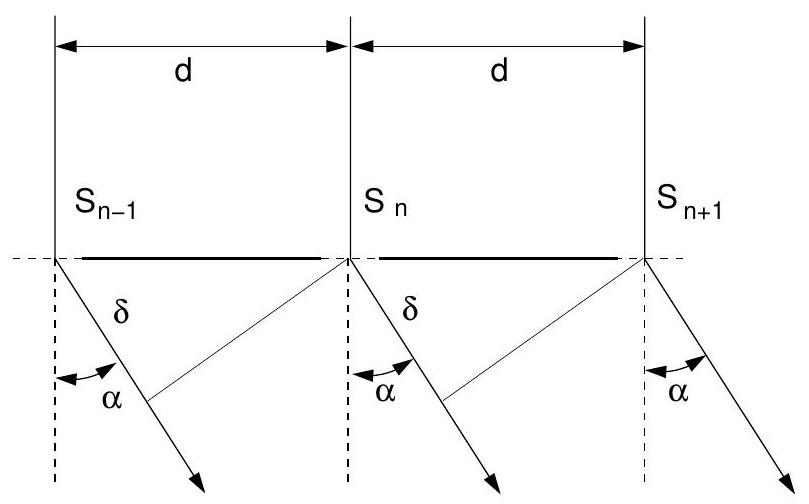
\includegraphics[max width=0.95\linewidth, center]{2024_12_20_2ef48a0ed8e6cd108eb0g-11}
		\caption{Schéma měření s difrakční mřížkou na průchod.}
	\end{figure}
	
	
	
	Z obr. 5 je zřejmé, že se tyto paprsky nesetkávají se stejnou fází. Označíme-li $S_{k}, S_{k+1}$ středy dvou sousedních štěrbin, pak jejich vzdálenost $d$ se nazývá mřížková konstanta a jejich střední paprsky mají dráhový rozdíl $d \sin \alpha$. Splñuje-li dráhový rozdíl $\delta$ podmínku
	
	
	\begin{equation}
		\delta=d \sin \alpha=m \lambda,
	\end{equation}
	
	
	zesilují se střední paprsky vycházející ze všech štěrbin. Parametr $m$ je řád maxima. Monochromatické světlo vytvoří tedy ve směrech daných úhly $\alpha_{1}, \alpha_{2}, \ldots$ maxima. Pro tyto úhly platí
	
	
	\begin{equation}
		\sin \alpha_{1}=\lambda / d, \sin \alpha_{2}=2 \lambda / d, \ldots, \sin \alpha_{r}=m \lambda / d
	\end{equation}
	
	
	Na základě vztahů 28 lze velmi přesně určit vlnovou délku světla.\\
	V našem experimentu bude zdrojem monochromatického světla He-Ne laser (vlnová délka $632,8 \mathrm{~nm}$ ), jehož světelný svazek je úzký a téměř nerozbíhavý. To umožňuje velmi jednoduché uspořádání: zdroj - mřížka - stínítko a místo měření úhlů $\alpha_{m}$ goniometrem určíme $\sin \alpha_{m}$ měřením délky stran v příslušném pravoúhlém trojúhelníku.\\
	\begin{figure}[H]
		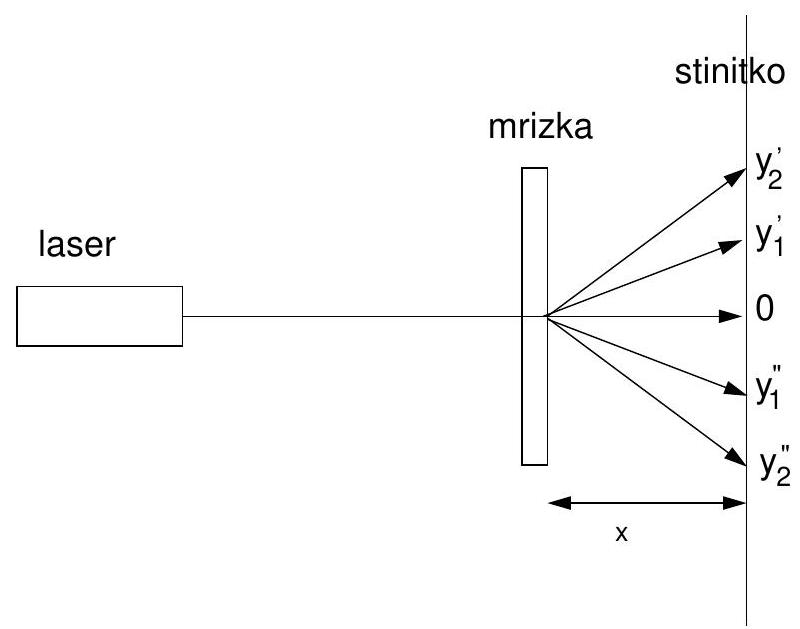
\includegraphics[max width=0.95\linewidth, center]{2024_12_20_2ef48a0ed8e6cd108eb0g-12}
		\caption{Schéma měření s difrakční mřížkou na průchod.}
	\end{figure}
	
	
	
	\section*{Uspořádání experimetu}
	Na optické lavici je umístěn He-Ne laser, optická mřížka a pozorovací stínítko s milimetrovým papírem, viz obr. 6. Mezi laser a mřížku vkládáme stínítko s malým otvorem pro světelný svazek, které zachytí paprsky vzniklé difrakcí při odrazu od mřížky a tím zamezíme nekontrolovanému pohybu laserového paprsku po laboratoři. Schéma uspořádání experimentu při pohledu shora je na obrázku.
	
	Při experimentu pozor - záření laseru je nebezpečné pro oko!\\
	Vzdálenost $x$ mezi mřížkou a stínítkem lze měnit a měřit ji pomocí stupnice na optické lavici. Protože vrypy na optické mřížce jsou orientovány svisle, budou difraktované svazky odchýleny vodorovně vlevo a vpravo od přímého (primárního) svazku. Označíme-li obecně vzdálenost místa dopadu přímého a difraktovaného paprsku jako $y$, bude
	
	\begin{equation}
		\sin \alpha_{m}=\frac{y_{m}}{\sqrt{y_{m}^{2}+x^{2}}} \quad m=1,2, \ldots
	\end{equation}
	
	
	Při měření nastavujeme různé vzdálenosti $x$ a pro každou hodnotu pak odečítáme na milimetrovém papíře stínítka polohy maxim prvního a druhého řádu vpravo $y_{1}^{\prime}, y_{2}^{\prime}$ a vlevo $y_{1}^{\prime \prime}, y_{2}^{\prime \prime}$ od primárního svazku. Odchylku paprsků na stínítku určíme jako průměr
	
	\begin{equation}
		y_{1}=\frac{y_{1}^{\prime}+y_{1}^{\prime \prime}}{2} \quad \text { a } \quad y_{2}=\frac{y_{2}^{\prime}+y_{2}^{\prime \prime}}{2}
	\end{equation}
	
	
	Dosazením 29 do 27 můžeme určit bud’ vlnovou délku světla $\lambda$, pokud známe vzdálenosti vrypů mřížky $d$, nebo vzdálenost vrypů $d$, resp. jejich hustotu $N$, pokud budeme znát vlnovou délku $\lambda$.
	
	\section*{Úkoly}
	\begin{enumerate}
		\item Pozorujte difrakční jev na stínítku a vzdálenost $x$ nastavte tak, aby bylo možno pozorovat dvě difrakční maxima po obou stranách stopy primárního svazku. Změřte polohu všech maxim a měření opakujte pro různé hodnoty $x$.
		\item Určete vzdálenost vrypů $d$ mřížky a jejich hustotu $N$. Zjištěnou hodnotu porovnejte s hodnotou uvedenou výrobcem mřížky. Vlnovou délku He-Ne laseru můžete nalézt též v tabulkách [3].
	\end{enumerate}
	
	
	
	
	
	
	
	
	
	
\end{multicols}
		\section{Měření}
		Z měření získáváme hodnoty $x_1, x_2$, formule 18 (při dosazení vlnové délky 531.2 laseru) nám dává tloušťku vrstvy d v nanometrech:
		
		\begin{center}
			\begin{tabular}{lll|lll|lll}
			\multicolumn{3}{c}{I. Poloha} & \multicolumn{3}{c}{II. Poloha} & \multicolumn{3}{c}{III. Poloha} \\ $x_2$    & $x_1$    &  d [nm]            & $x_2$    & $x_1$    &   d [nm]             & $x_2$     & $x_1$    &   d [nm]             \\ \hline
			89    & 219   & 107.94        & 192   & 483   & 105.58         & 151    & 397   & 101.02         \\
			80    & 209   & 101.67        & 193   & 473   & 108.37         & 143    & 383   & 99.17         \\
			82    & 212   & 102.73        & 180   & 475   & 100.65         & 158    & 397   & 105.70         \\
			85    & 215   & 105.00        & 175   & 452   & 102.83         & 171    & 387   & 117.35         \\ \hline
			&       & $104.3 \pm 1.4 $   &       &       & $104.4 \pm 1.7$   &        &       & $105 \pm 4$  
		\end{tabular}
		\end{center}
		
		
		\begin{multicols}{2}
			
		Lze předpokládat, že je tloušťka vrstvy v tomto případě ve všech polohách velmi podobná, i proto výsledky pro různé polohy nejsou překvapivé. Nicméně při samotném měření bylo poměrně složité hodnoty určit, jelikož rozhraní mezi jednotlivými pásy nebylo možné jasně rozlišit. Nicméně získáváme hodnotu
		$d = 104.8 \pm 1.4 \,\rm nm$
		
		\subsection{Určení indexu lomu vzduchu}
		
		Z analýzy nahrávek přechodu podtlak $\rightarrow$ atmosférický tlak získáváme hodnoty
		
		\begin{tabular}{l|lllll}
		N & 36 & 36 & 37 & 38 & 37
		\end{tabular} \\
		
		proto $\overline{N} = 36.8 \pm 0.37$
		
		a z formule 26 získáváme:
		
		$n_{vz} = 1.000244 \pm 0.000004$ 
		
		\subsection{Difrakce světla}
		Vzdálenost vrypů spočítáme z formule 27, 29, uvažujeme vlnovou délku He-Ne laseru, 632.8 nm:
		\begin{equation}
			d = m \lambda \frac{\sqrt{y_m^2 + x^2}}{y_m}
		\end{equation}
		získáváme:
		\end{multicols}
		\begin{center}
				\begin{tabular}{l|llll|llll}
			x [mm]   & $y_1$   & $y_2$    & $y_3$    & $y_4$    & $d_1$ [nm]          & $d_2$       & $d_3$       & $d_4$       \\ \hline
			59  & 13   & 28    & 47.25 & 79.35 & 2940.827497 & 2951.875 & 3036.962 & 3154.218 \\
			69  & 15   & 32    & 54    & 90.5  & 2978.868613 & 3008.141 & 3080.277 & 3182.979 \\
			79  & 17   & 35.5  & 59.5  & 100   & 3007.974427 & 3087.699 & 3155.498 & 3225.766 \\
			89  & 19   & 39.75 & 67.5  & 114   & 3030.961938 & 3103.455 & 3141.546 & 3211.229 \\
			99  & 21   & 43.75 & 74    & 124.5 & 3049.576705 & 3131.055 & 3170.845 & 3233.911 \\
			109 & 22.5 & 47.75 & 81    & 136   & 3130.195074 & 3154.068 & 3182.781 & 3243.844 \\
			119 & 24.5 & 52    & 87.5  & 148   & 3138.065136 & 3160.722 & 3204.643 & 3247.938 \\
			129 & 26   & 56    & 94    & 159   & 3202.79728  & 3178.254 & 3223.547 & 3259.495 \\
			139 & 28   & 60    & 101.5 & 171   & 3204.50149  & 3193.464 & 3219.126 & 3261.96  \\
			149 & 30   & 64    & 108   & 182   & 3205.978502 & 3206.783 & 3234.741 & 3271.265 \\
			159 & 32   & 68    & 115   & 194   & 3207.27091  & 3218.544 & 3239.322 & 3272.719 \\
			169 & 34   & 72    & 122   & 206   & 3208.411288 & 3229.005 & 3243.38  & 3274.004 \\
			179 & 36   & 76    & 129   & 216   & 3209.42497  & 3238.37  & 3246.999 & 3287.394 \\
			189 & 38   & 80    & 136   & 228   & 3210.331961 & 3246.802 & 3250.248 & 3287.788 \\
			199 & 40   & 84    & 143   & 240   & 3211.148261 & 3254.435 & 3253.181 & 3288.142 \\
			249 & 50   & 105   & 177   &       & 3214.250277 & 3257.211 & 3276.613 &          \\
			299 & 59   & 125   & 211   &       & 3268.73895  & 3281.216 & 3292.541 &          \\
			349 & 68   & 145   & 245   &       & 3308.826832 & 3298.619 & 3304.073 &          \\
			399 & 78   & 165   &       &       & 3298.288108 & 3311.813 &          &          \\
			449 & 88   & 186   &       &       & 3290.145428 & 3306.897 &          &          \\
			499 & 97.5 & 206   &       &       & 3299.880544 & 3316.665 &          &          \\
			549 & 106  & 226   &       &       & 3337.957421 & 3324.707 &          &          \\
			599 & 116  &       &       &       & 3328.357116 &          &          &        
		\end{tabular}\\
		pro optickou mřížku s třemi sty vrypy na milimetr a \\
		\begin{tabular}{l|ll|ll}
			x   & $y_1$    & $y_2$    & $d_1$       & $d_2$       \\
			39  & 20    & 57    & 1386.756 & 1533.489 \\
			49  & 24    & 69    & 1438.615 & 1552.26  \\
			59  & 28    & 80.5  & 1475.937 & 1569.125 \\
			69  & 32    & 92    & 1504.07  & 1582     \\
			79  & 36    & 102.5 & 1526.031 & 1597.881 \\
			89  & 40    & 114   & 1543.646 & 1605.615 \\
			99  & 44    & 125   & 1558.089 & 1614.453 \\
			109 & 48    & 137   & 1570.146 & 1617.302 \\
			119 & 52    & 148   & 1580.361 & 1623.969 \\
			129 & 56    & 160.5 & 1589.127 & 1623.719 \\
			139 & 60    & 172   & 1596.732 & 1627.214 \\
			149 & 64    & 183   & 1603.392 & 1632.052 \\
			159 & 68    & 195   & 1609.272 & 1632.993 \\
			169 & 72    & 207   & 1614.502 & 1633.825 \\
			179 & 76    & 217   & 1619.185 & 1640.617 \\
			189 & 80    & 230   & 1623.401 & 1638.087 \\
			199 & 85    & 242   & 1610.983 & 1638.549 \\
			249 & 105   &       & 1628.606 &          \\
			299 & 125.5 &       & 1635.046 &          \\
			349 & 146   &       & 1639.68  &          \\
			399 & 166.5 &       & 1643.175 &          \\
			449 & 186.5 &       & 1649.666 &          \\
			499 & 207   &       & 1651.49  &          \\
			549 & 227.5 &       & 1652.986 &          \\
			589 & 244   &       & 1653.423 &         
		\end{tabular}\\
		pro mřížku s šesti sty vrypy na milimetr.
		\end{center}
		\begin{multicols}{2}
		Z čehož získáváme:
		\begin{gather*}
			d_{300} = 3207 \pm 10 \,\mathrm{nm}\\
			d_{600} = 1594 \pm 10 \,\mathrm{nm}\\
			N_{300} = 311.8 \pm 1 \,\mathrm{mm^{-1}}\\
			N_{600} = 627 \pm 4 \,\mathrm{mm^{-1}}
		\end{gather*}
		
		\section{Závěr}
		Podařilo se nám splnit veškeré zadané úkoly a získat hodnoty hledaných veličin. Zatímco u indexu lomu vzduchu a hustoty vrypů máme referenční hodnoty, se kterými lze výsledek porovnat, u tloušťky vrstvy tomu tak není, tudíž úspěšnost ani přesnost tohoto měření nelze hodnotit. Ostatní veličiny však vyšly v očekávaných intervalech s poměrně přijatelnými odchylkami.
		
	
		

		
		
		
		
		
		% Nakonec nezapomeňte projet text programem vlna nebo vlnka, např.
		% 	vlna -m -l -n mojeuloha.tex
		% nebo zkontrolovat a opravit jednopísmenné předložky na koncích řádků ručně.
		\end{multicols}
\end{document}
